% ------------------------------------------------
%
%論文內容次序:
% 1.考試合格證明
% 2.中英文摘要(論文以中文撰寫者須附英文延伸摘要)
% 3.誌謝
% 4.目錄
% 5.表目錄
% 6.圖目錄
% 7.符號
% 8.主文
% 9.參考文獻
% 10.附錄
%
% 註: 參考文獻書寫注意事項:
% (1).
%    文學院之中文文獻依分類及年代順序排列。
%    其他學院所之文獻依英文姓氏第一個字母
%    (或中文姓氏第一個字筆劃)及年代順序排列。
%
% (2).
%    期刊文獻之書寫依序為:
%        姓名、文章名稱、期刊名、卷別、期別、頁別、年代。
%
% (3).
%    書寫之文獻依序為:
%        姓名、書名、出版商名、出版地、頁別、年代。
%
% ------------------------------------------------

% 封面內頁 Inner Cover
%
% 封面: 顯示所有封面內容, 沒有學校Logo
%     主要用在印刷版, 如精裝版 或 平裝版
%     (使用cover.tex來產生)
%
% 內頁: 顯示所有封面內容, 沒有學校Logo
%     主要用在電子版 + 印刷版
%
% 只要是印刷版, 不論是精裝版或平裝版, 都是 封面 (殼/皮) + 內頁.
% 只有在電子版時, 第一頁就是封面內頁.

\DisplayInnerCover

% ------------------------------------------------

% 學位考試論文證明書
\DisplayOral

% ------------------------------------------------

% 摘要 Abstract
% 除了外籍生, 本地生和僑生都是要編寫中文和英文摘要
% 論文以中文撰寫須以英文補寫 800 至 1200 字數的英文延伸摘要 (Extended Abstract)
% 詳細可看附件的學校要求或看example中的英文延伸摘要

%% ------------------------------------------------
\StartAbstractChi
% ------------------------------------------------

這是國立成功大學碩博士用畢業論文的LaTex模板. 這模板是使用學校最新的畢業論文要求來設計(參考: 附錄 - 撰寫論文須知 P.\RefPage{appendix:thesis-spec}).

這模板的目標是為了提供學生可以使用LaTex來寫畢業論文. 但是各系所有各自的格式, 故請在使用前先留意自己的系所有沒有格式要求 (參考: 附錄 - 可使用的系所 P.\RefPage{appendix:acceptable-dept}). 如果沒有, 則這模板應該用來使用; 否則要看系所上的格式, 是否跟這模板有相同的寫法.

這模板的內容是我參考了我所拿到的一些畢業論文的LaTex模板設計, 跟系上老師的一些對話, 和上課所聽得出的結論和想法而寫出的, 所以某些地方會帶有我們濃郁的資工系味道. 另外如果有任何的老師 (不論本系外系)可以提供一些意見或想法的話, 我會十分感謝的.

這模板盡量以全自動化方式去處理一些不用你去煩惱的部份, 如排版和設計. 只留下要你去填寫的部份, 所以只要選擇和填入你的內容, 就能得到一份符合學校要求的畢業論文.

最後, 希望你使用愉快.

% ------------------------------------------------
% 如果在conf.tex中的\SetAbstractChiKeywords有設定任何的關鍵字,
% 那中文版的關鍵字會在使用\EndAbstractChi後同時顯示出來.
\EndAbstractChi
% ------------------------------------------------
             % 中文版
\input{./context/abstract/eng}             % 英文版
%\input{./context/abstract/extended}        % 英文延伸摘要

% ------------------------------------------------

% 誌謝 Acknowledgments
% 誌謝正常應該只要寫一種版本就可,
% 提供2種以自行選擇所顯示的語言.
% 2種同時編寫都是可以的.

%% ------------------------------------------------
\StartAbstractChi
% ------------------------------------------------

這是國立成功大學碩博士用畢業論文的LaTex模板. 這模板是使用學校最新的畢業論文要求來設計(參考: 附錄 - 撰寫論文須知 P.\RefPage{appendix:thesis-spec}).

這模板的目標是為了提供學生可以使用LaTex來寫畢業論文. 但是各系所有各自的格式, 故請在使用前先留意自己的系所有沒有格式要求 (參考: 附錄 - 可使用的系所 P.\RefPage{appendix:acceptable-dept}). 如果沒有, 則這模板應該用來使用; 否則要看系所上的格式, 是否跟這模板有相同的寫法.

這模板的內容是我參考了我所拿到的一些畢業論文的LaTex模板設計, 跟系上老師的一些對話, 和上課所聽得出的結論和想法而寫出的, 所以某些地方會帶有我們濃郁的資工系味道. 另外如果有任何的老師 (不論本系外系)可以提供一些意見或想法的話, 我會十分感謝的.

這模板盡量以全自動化方式去處理一些不用你去煩惱的部份, 如排版和設計. 只留下要你去填寫的部份, 所以只要選擇和填入你的內容, 就能得到一份符合學校要求的畢業論文.

最後, 希望你使用愉快.

% ------------------------------------------------
% 如果在conf.tex中的\SetAbstractChiKeywords有設定任何的關鍵字,
% 那中文版的關鍵字會在使用\EndAbstractChi後同時顯示出來.
\EndAbstractChi
% ------------------------------------------------
             % 中文版
\input{./context/acknowledgments/eng}             % 英文版

% ------------------------------------------------

% 目錄 (內容, 圖表和圖片) Index of contents, tables and figures.
% 內容會自動產生 The indices will generate in automate.
\DisplayIndex                 % 顯示索引
\DisplayTablesIndex   % 顯示表格索引
\DisplayFiguresIndex  % 顯示圖片索引

% ------------------------------------------------

% Nomenclature
\input{./example/nomenclature/nomenclature}

% ------------------------------------------------

% Introduction chapter
% ------------------------------------------------
\StartChapter{Introduction}{chapter:introduction}
% ------------------------------------------------

這是國立成功大學碩博士用畢業論文的LaTex模板. 本模板是使用學校最新的畢業論文要求來設計(參考: 附錄 - 撰寫論文須知 P.\RefPage{appendix:thesis-spec}).

雖然本模板的目標是為了提供學生可以使用LaTex來寫畢業論文. 但是各系所有各自的格式, 所以做了一個表列出已知的系所情況(參考: 附錄 - 可使用的系所 P.\RefPage{appendix:acceptable-dept}), 故請在使用前先留意自己的系所有沒有格式要求. 如果沒有, 則本模板應該是可以用來使用; 否則要看系所上的格式, 是否跟本模板有相同的寫法.

本模板分以下幾個主要部份來進行教學:

\begin{enumerate}
  \item 本模板的架構設計
  \item 設定本模板的一些資料以轉成你的論文
  \item 介紹LaTex和本模板所提供的語法
  \item 最後有一個chapter為``老師們的話''(Chap.\RefTo{chapter:words-from-professor})寫了一些老師對論文的想法和意見, 以供同學們留意
\end{enumerate}

同學們只要閱讀完後, 把部份的檔案直接copy和修改內容, 應該很快就能上手本模板去寫自己的論文.

另外在附錄(Appendix)附上了一些重要的學校的文件, 由於本模板很接近完善, 故直接使用本模板後可不需再閱過學校相關規定之文件, 所以該類文件置於此僅為備考用.

% ------------------------------------------------
\newpage

\begin{description}
  \item[版權 License]\hfill\\
  詳細請看`LICENSE'這檔案中的條款說明.\\

  \InsertFigure
    [scale=0.8,
      caption={CC Attribution-NonCommercial-ShareAlike License},
      label={fig:appendix:by-nc}]
    {./example/introduction/pic/by-nc-sa.png}

    本著作(ncku-thesis-template-latex\RefBib{web:this-project:github})採用創用 CC 姓名標示-非商業性-相同方式分享 4.0 授權條款.

    This work(ncku-thesis-template-latex\RefBib{web:this-project:github}) is licensed under Creative Commons Attribution-NonCommercial-ShareAlike 4.0 International License.\\

  而本模板所使用到的國立成功大學浮水印則由國立成功大學擁有\textbf{所有}相關的權利. 故如使用這浮水印到論文以外的應用, 請跟`成大圖書館 系統管理組-數位論文小組'聯絡.\\

  \item[版本修改 ChangeLog]\hfill\\
  詳細請看`ChangeLog.md'這檔案中的說明.
\end{description}

% ------------------------------------------------
\EndChapter
% ------------------------------------------------


% Objective chapter
%% ------------------------------------------------
\StartChapter{Objective}{chapter:objective}
% ------------------------------------------------

\StartSection{起因}

做這個模板的原因其實很簡單:

\begin{enumerate}
  \item
  {
    去投國外paper時, 對方可能會要求使用LaTeX, 所以未來要懂LaTeX是不意外的.
  } % End of \item{}

  \item
  {
    想拿LaTeX來寫畢業論文, 卻發現學校只提供Mircosoft Word模板, 但卻沒有提供LaTeX的, 所以證明本模板對學校是有存在價值的.
  } % End of \item{}

  \item
  {
    因為看到發現台灣科技大學\RefBib{web:latex:template:ntust}, 台灣大學\RefBib{web:latex:template:ntu}, 元智大學\RefBib{web:latex:yzu}都能找到LaTeX的模板, 連大陸那邊都有一些學校有在提供, 更不用說國外的學校.

    那些學校的畢業論文模板不只提供是Mircosoft Word版本(.doc), 是會連LaTex(.tex)版本都有, 而我們學校卻沒有. 唯一我們學校在Google上找到的有提到的卻是數學系系網頁上的功能\RefBib{web:latex:ncku_math_introduction}和建在數學系上的一個討論區\RefBib{web:latex:ncku_math_forum}.
  } % End of \item{}

  \item
  {
    因為學校對Phd跟Master的畢業論文要求是同一個格式, 所以如果完成後對學校任何學生應該都有其好處.

    對大家都有多一個選擇來寫畢業論文, 而不是被限在使用Mircosoft Word來寫.
  } % End of \item{}

  \item
  {
    經過詢問我們資訊工程系(CSIE)的系上一些老師後, 意外發現原來某些實驗室其實已經有各自的版本存在, 但每個版本都有各自的優缺點, 例如:

    \begin{enumerate}

      \item
      {
        新的使用者或接手的人不容易修改或使用.
      } % End of \item{}

      \item
      {
        或是需要安裝的步驟十分麻煩 (e.g cwTeX\RefBib{web:latex:cwtex}).
      } % End of \item{}

      \item
      {
        另外有一些因為是只針對英文版本, 沒有考量在編寫或初稿時會有中英混雜的時候, 故這時候中英文的內容要分開編寫和產生 (學校又要求, 英文內容的論文要同時有中文論文名字等), 所以需要把整個論文分開成不同的檔案.
      } % End of \item{}
    \end{enumerate}
  } % End of \item{}
\end{enumerate}

% ------------------------------------------------

%\newpage
\StartSection{目標}
所以為了解決以上的問題, 這個模板針對了好幾點來處理:

\begin{enumerate}

  \item
  {
    把本模板做到連笨蛋都可以很快懂得使用(所謂的Books for Dummies), 所以只留下使用者要填寫的部份外, 其他都交由模板去負責.
  } % End of \item{}

  \item
  {
    希望做到使用者只讀這份模板, 就會懂得去修改和寫自己所需的內容(所謂的Self-contained. 但其實是不太可能的, 因為LaTex的使用手冊就算寫成一本幾百頁的書, 都可以缺少很多東西), 所以會同時提供很基本使用LaTex的方式, 和填寫本模板步驟.
  } % End of \item{}

  \item
  {
    希望一份模板, 能同時應用在中文或是英文版本, 只要修改內容和一些的設定.
  } % End of \item{}

  \item
  {
    把本模板open source, 讓以後任何的同學們都可以使用和修改, 以合適當時的需求.
  } % End of \item{}

\end{enumerate}

而選擇使用XeLaTex的原因, 是經過分析cwTeX, CJK和XeLaTex後. 發現cwTeX的寫法太糟, 要背多新一種語法, 而且安裝複雜\RefBib{web:latex:cwtex}; 而CJK有一定程度的設定才能在整個論文中自由使用, 感覺設定麻煩而不太能笨蛋化來用, 所以放棄選用; 故最後選用最簡單加一些包裝, 就可以簡單使用中英混合的XeLaTex.

% ------------------------------------------------

\StartSection{缺點}
但是同樣任何東西都會有缺點, 故本模板都不意外:

\begin{enumerate}

  \item
  {
    本模板是以台灣國立成功大學所最新訂下的畢業論文要求(參考: 附錄 - 撰寫論文須知 P.\RefPage{appendix:thesis-spec})來設計, 所以不一定能對非本校的人有用.
  } % End of \item{}

  \item
  {
    對沒有程式基礎, 只會用Mircosoft Word的人來講, 可能會在修改或使用上會十分吃力.
  } % End of \item{}

  \item
  {
    因為我針對某些使用者不用去接觸的部份, 進行了大量的包裝(Wrapping), 所以如果懂得LaTex的人可能會覺得我破壞了LaTex的語法. 但是本模板是針對笨蛋化和全自動, 我相信對不熟LaTex的人來講, 才不管這問題 (如同一般理論派和應用派的差別, 在意的方向完全不一樣).
  } % End of \item{}

%  \newpage
  \item
  {
    某些包裝出來的語法, 可能會在一些情況下會產生衝突而令LaTex不接受, 這時候有2種做法:
    \begin{enumerate}
      \item
      {
        不使用某些寫法, 例如已知的`\verb|\InsertFigure|'沒法被包在Table, minipage或framebox中.
      } % End of \item{}

      \item
      {
        如真的要使用那些情況, 那就不要使用模板提供的語法, 而直接去寫LaTex原版的語法.
      } % End of \item{}
    \end{enumerate}
  } % End of \item{}
\end{enumerate}

% ------------------------------------------------

\StartSection{總結}

以上是個人對這份模板的一些想法和起源, 同時希望本模板能對你提供到一些幫助.

% ------------------------------------------------
\EndChapter
% ------------------------------------------------


% Related Work chapter
\input{./context/related-work/related-work}

% Algorithm chapter
%\input{./context/algorithm/algorithm}

% Performance chapter
%\input{./context/performance/performance}

% Conclusion chapter
\input{./context/conclusion/conclusion}

% Future work chapter
%\input{./context/future-work/future-work}

% ------------------------------------------------

% 參考文獻 References
% References and bibliography

% Import the files that contain your references.
% If you set some references file,
% you need to use at least one cite to make LaTex work.

\ReferencesFiles{./example/references/paper}{./example/references/misc}{./example/references/book}


% ------------------------------------------------

% 附錄 Appendix
%% ------------------------------------------------
\StartAppendix
% ------------------------------------------------

% ------------------------------------------------
\StartChapter{可使用這模板的系所}{appendix:acceptable-dept}
% ------------------------------------------------

這邊列出一些\textbf{應該可使用}或\textbf{不可使用}這模板的系所名字, 這表可能會有不正確, 所以還是先問系辦確定會比較好. \\

因為這名單都是靠網路上能找多少而得出的結果, 而如果沒有分類的話, 很高機會是使用圖書館的要求 (即是可使用本模板). \\

而如果這表名單中沒有顯示你的系所, 但你已經\textbf{知道}是否能使用, 請告知以供更新.

\clearpage

% ------------------------------------------------
\section{應該可使用}

  可使用的原因幾乎都是系所自己沒有特殊要求, 所以直接使用圖書館的要求, 而本模板就是跟隨圖書館所定下的要求來設計.

  \InsertTable
    [caption={應該可使用的系所},
      label={table:acceptable-dept:acceptable}]
    {
      \begin{tabular}{|l|l|}
      \hline
      資訊工程學系 & Department of Computer Science and Information Engineering \\ \hline
      \end{tabular}
    } % End of \InsertTable

% ------------------------------------------------
\section{應該不可使用}

  不可使用的原因是那系所已經有提供一份樣版出來, 而那份樣版的要求有沒有跟本模板一樣設計, 這個就不作詳細分析. 故如果已經有樣版, 那我就會自動把它們分類成\textit{無法使用這本模板}比較好, 但如果分類錯誤, 請告知.

  \InsertTable
    [caption={應該不可使用的系所},
      label={table:acceptable-dept:unacceptable}]
    {
      \begin{tabular}{|l|l|l|}
      \hline
      生物科技研究所 & Institute of Biotechnology & \href{www.biotech.ncku.edu.tw/files/archive/331_4b79187a.doc}{Link} \\ \hline
      體育健康與休閒研究所 & \begin{tabular}[c]{@{}l@{}}Institute of Physical Education\\ Health and Leisure Studies\end{tabular} & \href{www.ncku.edu.tw/~deprb/docs/Thesis\%20Regulation\%20.doc}{Link} \\ \hline
      \end{tabular}
    } % End of \InsertTable

% ------------------------------------------------
\EndChapter
% ------------------------------------------------

% ------------------------------------------------
\StartChapter{繳交流程說明}
% ------------------------------------------------

這部份資料來源是使用'電子學位論文服務'提供的'電子學位論文服務流程說明圖'\RefBib{web:lib:submit-flow}和'繳交論文全文電子檔案說明'\RefBib{web:lib:submit-file}.\\

\setboolean{@twoside}{false}
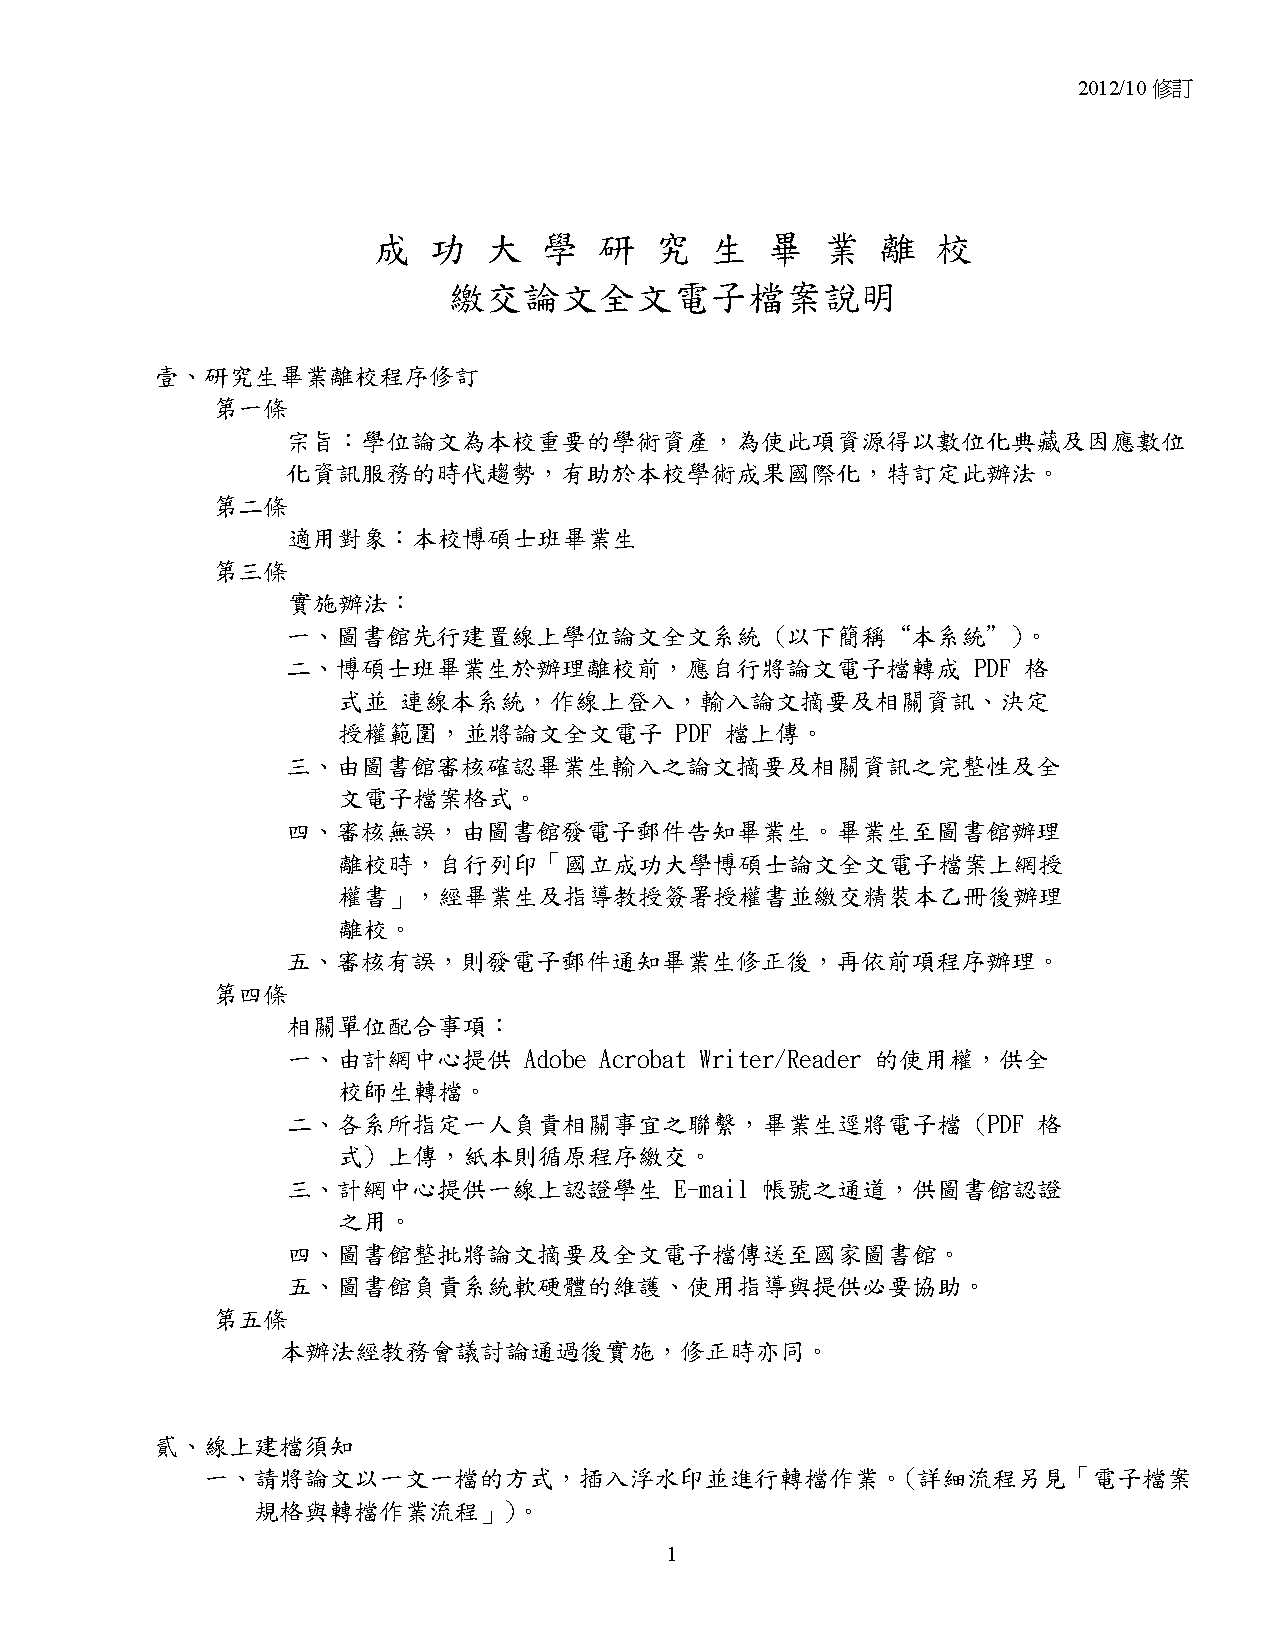
\includepdf[pages=-]{./example/appendix/pdf/2012050004-a.pdf}
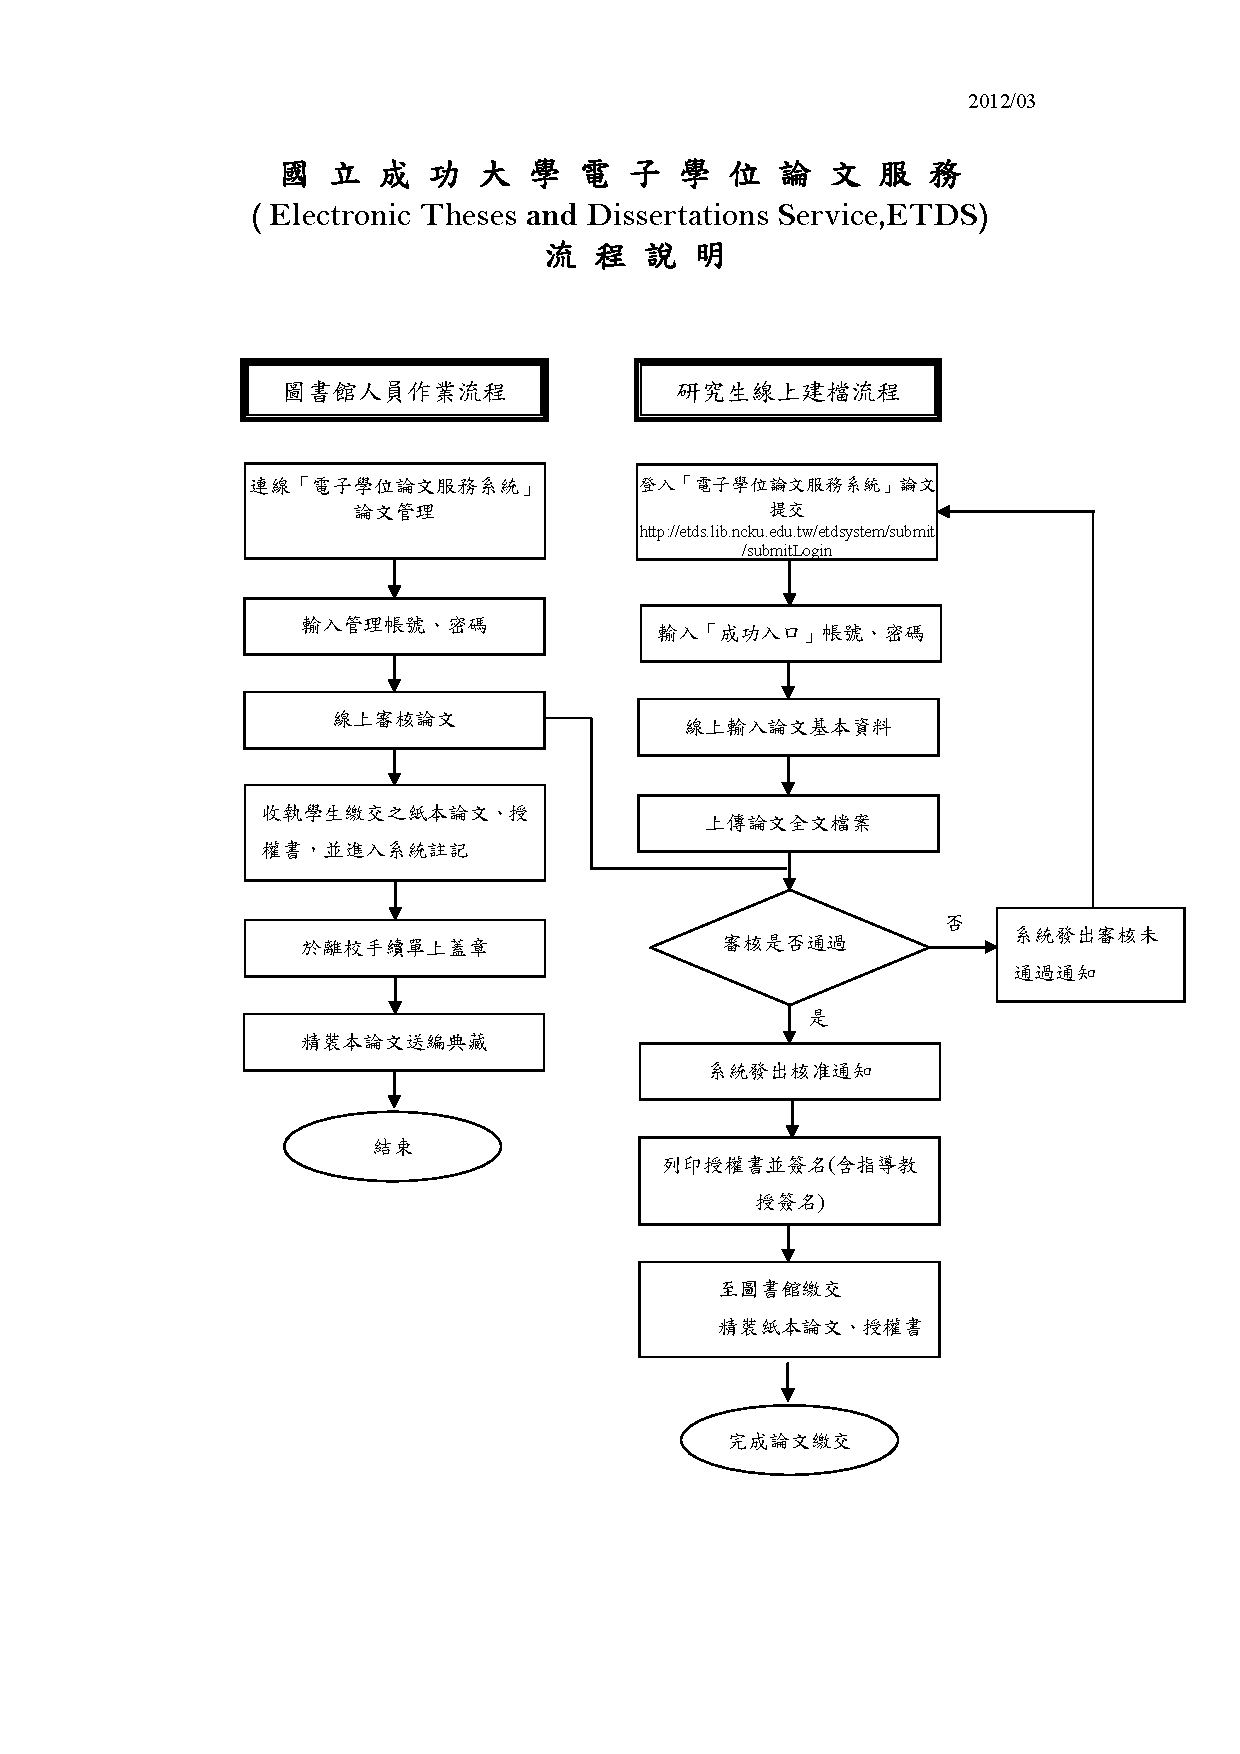
\includepdf[pages=-]{./example/appendix/pdf/2012050006-a.pdf}

% ------------------------------------------------
\EndChapter
% ------------------------------------------------

% ------------------------------------------------
\StartChapter{各系所博碩士撰寫論文須知}{appendix:thesis-spec}
% ------------------------------------------------

這部份資料來源是使用'電子學位論文服務'提供'國立成功大學博碩士學位論文格式規範'\RefBib{web:ncku:thesis-need-to-know}.\\

\setboolean{@twoside}{false}
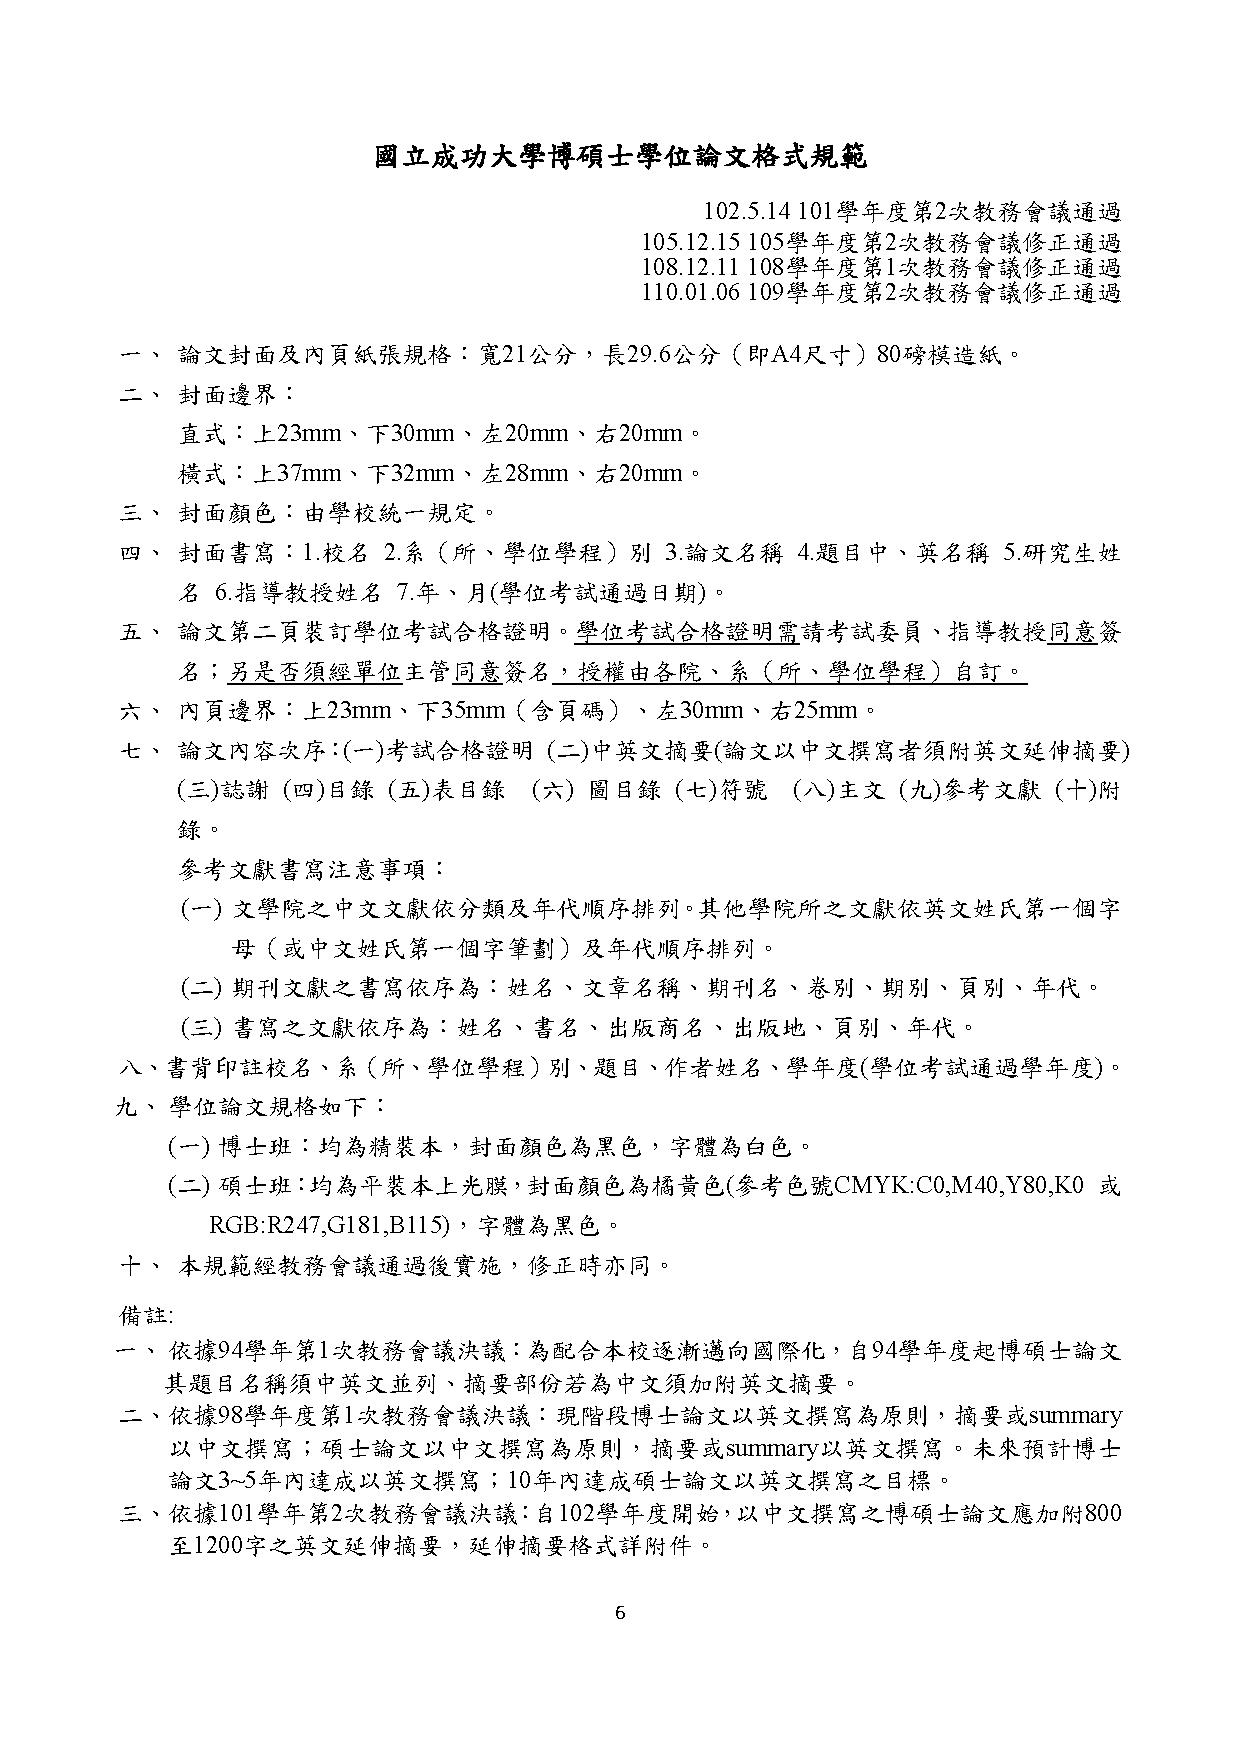
\includepdf[pages=-]{./example/appendix/pdf/thesis-spec-a.pdf}

% ------------------------------------------------
\EndChapter
% ------------------------------------------------

% ------------------------------------------------
\StartChapter{電子論文上傳前檢查事項}{appendix:e-paper_upload}
% ------------------------------------------------

這部份資料來源是使用'電子學位論文服務'中的'電子論文上傳前檢查事項'的'2012090001.pdf'\RefBib{web:lib:upload-things-check}.\\

\setboolean{@twoside}{false}
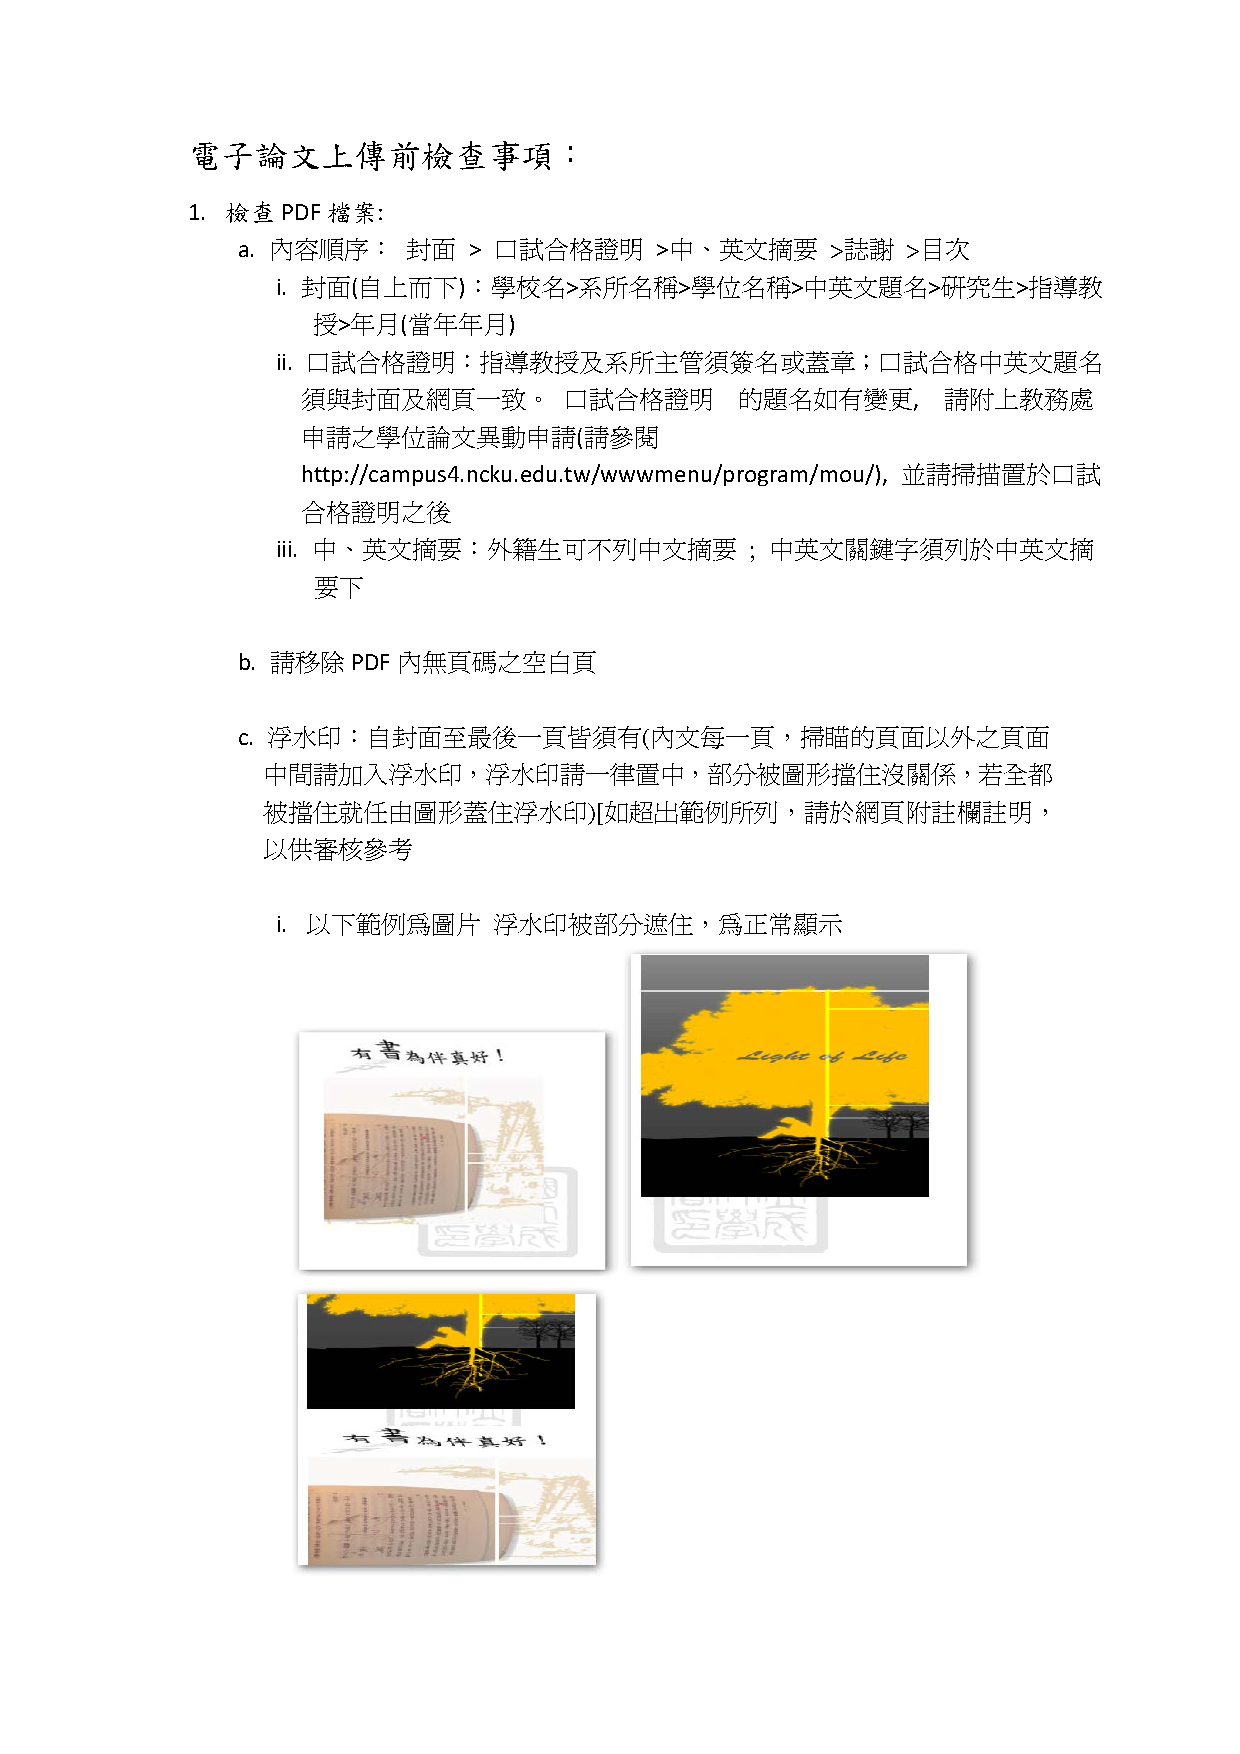
\includepdf[pages=-]{./example/appendix/pdf/2012090001-a.pdf}

% ------------------------------------------------
\EndChapter
% ------------------------------------------------

% ------------------------------------------------
\StartChapter{論文提交說明}{appendix:e-paper_upload_ppt}
% ------------------------------------------------

這部份資料來源是使用'電子學位論文服務'提供的 '2016論文提交說明簡報檔'\RefBib{web:lib:2016-submit-ppt} 修改而成的, 只抽出使用本模版後, 還要做什麼的行為.\\

\setboolean{@twoside}{false}
\includepdf[pages=-]{./example/appendix/pdf/2012050003-short-a}

% ------------------------------------------------
\EndChapter
% ------------------------------------------------

% ------------------------------------------------
\StartChapter{口試注意事項}
% ------------------------------------------------

這部份資料來源是使用本系資訊工程研究所系辦所提供的資料, 雖然內容主要針對本系, 但某些內容都是適合非本系的同學們.

\setboolean{@twoside}{false}
\includepdf[pages=-]{./example/appendix/pdf/oral-1040616-a.pdf}

% ------------------------------------------------
\EndChapter
% ------------------------------------------------

% ------------------------------------------------
\StartChapter{常見問題Q\&A}{appendix:faq}
% ------------------------------------------------

這部份資料來源是使用'電子學位論文服務'提供的'FAQ'\RefBib{web:lib:ETDS-QA}, 用來補充其他Appendix沒提到的一些情報.\\

\setboolean{@twoside}{false}
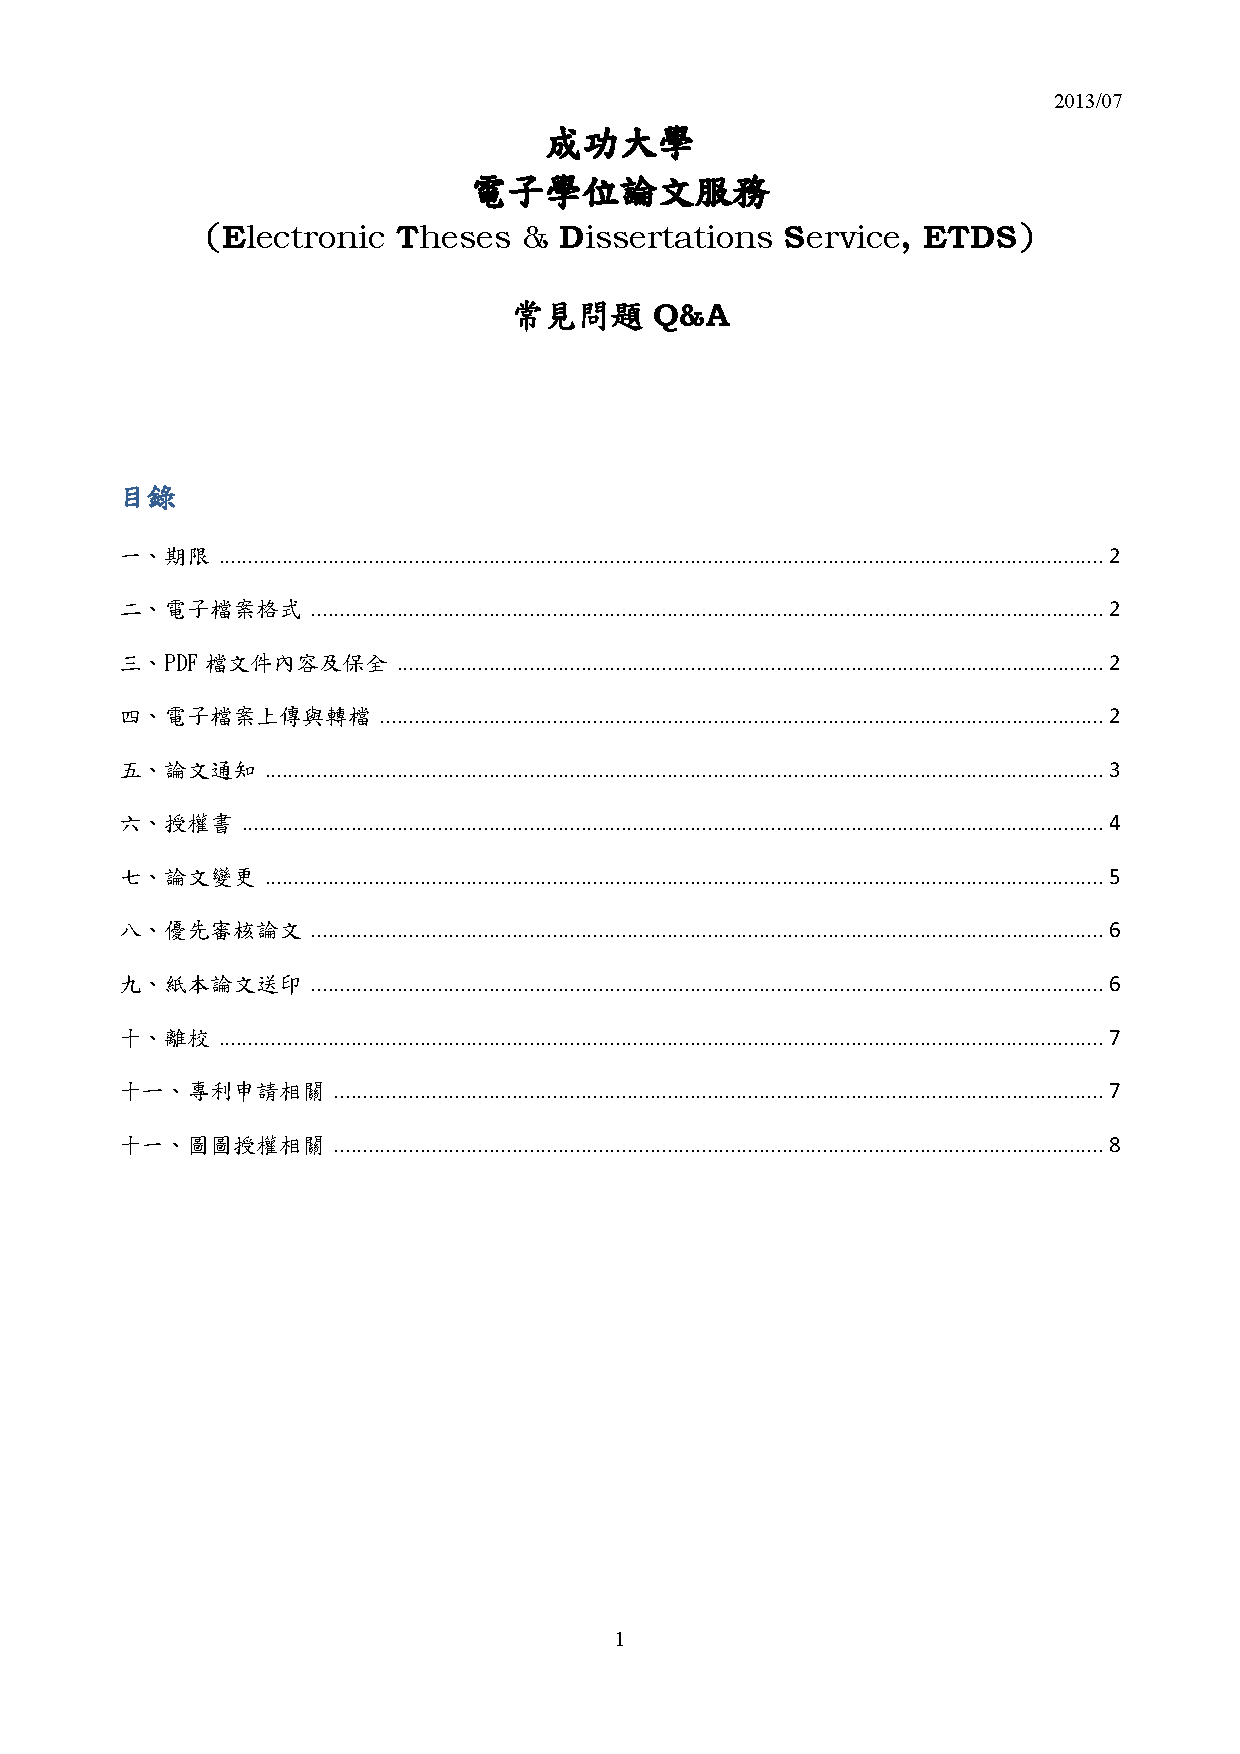
\includepdf[pages=-]{./example/appendix/pdf/2012050009-a.pdf}

% ------------------------------------------------
\EndChapter
% ------------------------------------------------

\input{./example/appendix/unicode-symbols}

% ------------------------------------------------
\EndAppendix
% ------------------------------------------------


% ------------------------------------------------
